\documentclass{article}
\usepackage[margin=1in]{geometry}
\usepackage{graphicx}
\usepackage{hyperref}
\hypersetup{hidelinks}
\usepackage{xcolor}
\usepackage{booktabs} % put this in your preamble
\usepackage{natbib}
\setcitestyle{round}
\bibliographystyle{unsrtnat}
\usepackage{amsmath}

\title{Smart eDNA sampling strategies: Species spatial autocorrelation can guide efficient marine survey design}

\author{Gledis Guri$^1$\textbf{*} \and
Ryan P. Kelly$^1$ \and
Ole Shelton2$^2*$ \and
Krista M. Nichols$^2$ \and others}

\date{\today}

\begin{document}

\maketitle

\section*{}

\begin{center}
\begin{tabular}{ll}
1 & School of Marine and Environmental Affairs, University of Washington, Seattle, Washington, USA \\
2 & Conservation Biology Division, Northwest Fisheries Science Center, NOAA Fisheries, \\
 & \qquad 2715 Montlake Blvd E. Seattle, Washington, USA \\
\hline
& corresponding author \textbf{gguri@uw.edu}
\end{tabular}
\end{center}

\section*{Abstract}

\textbf{Keywords}: 















\section{Introduction}
Marine sampling efficiency plays a critical role in collecting sufficient and representative samples to accurately assess species distributions, forming the foundation for sound fisheries management and stock assessment protocols. In stock assessment contexts, determining the appropriate sample size is vital for reliable estimation of population parameters including abundance, demographic structure, and spatial distribution patterns. This process must balance the need for sufficient data for detecting trends and changes in population while also ensuring that incurring unnecessary costs or effort are minimized. Excessive sampling can lead to redundant data -- multiple samples that gives the exact same information - whereas insufficient sampling risks overlooking critical patterns and producing unreliable estimates. Identifying the point at which sampling efficiency is optimized is crucial therefore, efficient sampling strategies are designed to capture the spatial variability of marine communities, allowing researchers to infer ecological traits such as habitat preferences and ecological niches without making a big dent on the budget.

While increased sampling intensity generally reduces variance in population estimates and improves the precision of spatial pattern detection, this relationship exhibits diminishing returns where beyond a certain threshold, additional sampling effort produces marginal gains in statistical precision that may not justify the associated costs and logistical demands. The optimal sampling intensity occurs at the point where incremental improvements in precision or information content become disproportionately small relative to the required investment of resources and effort. This principle guides the development of cost-effective sampling strategies that maximize analytical power while minimizing operational expenditure.

In ecological and fisheries research, Gaussian Process (GP) models have been widely adopted to capture spatial and environmental variation in species distributions. For instance, xxx. GP models provide a powerful and flexible framework for describing spatial and environmental patterns without assuming a fixed functional form between predictors and responses. These examples highlight the versatility of GP models in ecological applications, enabling researchers to infer complex, nonlinear relationships between species occurrence, abundance, and environmental covariates while quantifying uncertainty in predictions. This approach is grounded in the assumption that species distributions and abundances change in a smooth and continuous manner, reflecting correlated responses to spatial, environmental, and biological covariates.

At the core of a GP is the idea that observations made at similar locations or under similar covariates should yield similar outcomes. This relationship is quantified through a covariance function, or kernel, which governs how the correlation between two points $x$ and $x\prime$ decays with increasing distance. The kernel defines the smoothness of the modeled across the covariates. One of the most influential parameters in this context is the length-scale, which represents the characteristic distance over which correlation between points remains strong. Large length-scales indicate that the modeled process changes gradually, with nearby points remaining highly correlated even over broad spatial extents or environmental conditions, whereas small length-scales imply rapid variation and weak correlation beyond short distances and environmental conditions. Spatially, this mathematical framework captures an essential ecological principle: species tend to form one or more areas of high concentration - "hotspots" - where individuals aggregate densely. As distance increases from these central areas, population density gradually declines in a smooth, continuous manner. The distribution of a species at various locations can be expressed as:
\begin{align}
Y &\sim MVN (\mu,k(x,x\prime))\\
k(x, x\prime) &= \alpha^2 \exp\left(-\frac{(x - x\prime)^2}{2\rho^2}\right) + \sigma^2
\end{align}
where Y is the vector of observed abundance or density of the species (spatial field) across all sampled locations with a global mean abundance $\mu$ and covariate matrix k of coordinate $x$ and $x\prime$. The covariate matrix is the most important part of the GP as it determines the (spatial or environmental) autocorrelation of the species distribution where $\alpha$ is the amplitude of the $x$-$x\prime$ correlation, $\rho$ is the length-scale parameter meaning the correlation (in $x$-$x\prime$ units) where the signal fades out, and $\sigma$ is the noise in nature. Species with small autocorrelation ($\rho$) values exhibit rapidly changing abundance patterns that vary sharply across space and environmental gradients, indicating highly localized distributions with distinct boundaries between favorable and unfavorable conditions. Conversely, species with large $\rho$ values display smoothly varying abundances that remain correlated over broader spatial and environmental scales, suggesting gradual transitions in response to environmental heterogeneity and broader ecological niches.

The emergence of environmental DNA (eDNA) sampling has revolutionized marine monitoring capabilities, offering a non-invasive method to detect species presence and estimate relative abundance. In contrast to traditional survey techniques that are typically species-specific or require separate sampling efforts for different taxa, eDNA enables simultaneous, multi-species detection from a single water sample. This holistic approach allows for a more comprehensive assessment of community composition while substantially reducing field effort and disturbance. Additionally, while conventional methods detect organisms directly at the point of capture or observation, eDNA signals integrate information from surrounding areas through processes of DNA transport and decay. This spatial integration effect means that adjacent eDNA samples may contain overlapping information, making the question of optimal spatial sampling resolution even more critical. Due to the spatiotemporal integration in eDNA signals -- DNA signal from organisms located at varying distances from the sampling site and at different time points prior to collection - an additional layer of spatial autocorrelation is introduced beyond what would be expected from species distribution patterns alone. Consequently, when applying Gaussian Process models to eDNA data, the spatial autocorrelation parameter inherently captures both the natural clustering patterns of species distributions and the physical processes that govern DNA dispersal and decay in the marine environment. Without concurrent independent sampling methods such as trawl surveys or acoustic monitoring to provide direct measures of local abundance, these two fundamental processes - biological smoothness and spatiotemporal eDNA integration - cannot be empirically separated and are therefore represented as a single integrated parameter within the modeling framework.


In simple terms, knowing the spatial autocorrelation of species distributions can provide a quantitative basis for optimizing sampling effort - species exhibiting high spatial autocorrelation should require fewer samples to capture their distribution patterns due to their extended spatial coherence. In this study, we aim to evaluate how spatial autocorrelation in relation to sampling effort (number of smaples deployed) influences the efficiency of marine sampling strategies of eDNA metabarcoding observation methods. Specifically, we quantify the effect of sampling effort on (i) estimating the spatial autocorrelation (typically used for understanding ecological niches), (ii) estimatig the global mean (typically used for conservation and stock assessment), and (iii) the predictive precision of species abundance and distributions (typically used for species distribution inferneces). In this formulation, we focus exclusively on spatial coordinates (latitude and longitude) as covariates to isolate the effects of spatial structure from environmental or biological drivers. However, the same GP framework can be extended to include additional covariates such as temperature, salinity, depth, or even biotic interactions like species competition and trophic relationships. By explicitly quantifying the trade-off between spatial autocorrelation, sample size, and prediction accuracy, this study seeks to identify thresholds of sampling effort that maximize information gain and minimize redundancy—offering a principled, quantitative foundation for designing efficient marine spatial surveys.
























\section{Materials and methods}

\subsection{Real-world eDNA data}
We analyzed eDNA concentration data collected from marine environments, as detailed in \citet[][in review]{guri2025}. This dataset includes eDNA measurements from 358 spatially distributed sampling sites across multiple depth layers spanning a broad latitudinal and longitudinal gradient along the U.S. West Coast, covering an approximate spatial extent of 123.53° - 125.93° W (243 - 461 km UTM eastings; range of 218 km) and 38.36° - 48.46° N (4249 - 5367 km UTM northings; range 1118 km), corresponding to a region from central California to northern Washington. . Samples were processed using metabarcoding with the MiFish U universal primer, enabling identification of fish species and quantification of eDNA abundance through calibration with a mock community and reference species \citep[][in review]{guri2025}.

Environmental DNA samples were collected during the Joint U.S.-Canada Integrated Ecosystem and Pacific Hake Acoustic-Trawl Survey aboard the NOAA ship Bell M. Shimada in summer 2019 \citep{deblois2020}. At each site, seawater (10 L) was collected using Niskin bottles mounted on a CTD rosette system, targeting five depths (0, 50, 150, 300, and 500 m). From each bottle, 2.5 L of seawater was immediately filtered onboard through sterile 47 mm mixed cellulose ester filters (1 $\mu$m pore size) to capture suspended eDNA. Filters were preserved and DNA was extracted using a phase-lock phenol-chloroform protocol, following established methods \citep{ramon-laca2021, shelton2022}. 

Samples were metabarcoded, libraries were prepared with the MiFish U universal primer set \citep{miya2015}, targeting a ~170 bp fragment of the mitochondrial 12S rRNA gene. Sequencing was performed on an Illumina MiSeq platform (2x150 bp paired-end) at the University of Washington Genomics Core. Raw sequence reads were processed using the DADA2 pipeline \citep{callahan2016} to generate amplicon sequence variants (ASVs), which were taxonomically assigned using a custom reference database from NCBI GenBank and BOLD Systems. Species-specific eDNA concentrations were estimated by normalizing ASV read counts to total reads per sample and calibrating against qPCR-derived abundances for target species. After subsequent filtering a total of 358 samples were used in a joint model where together with a mock community correcting for amplification bias and qPCR of pacific hake to estimate absolute eDNA abundance for 12 fish species \citep[][in review]{guri2025}.


\subsection{Simulated eDNA data}
A common approach to evaluating sampling efficiency has been retrospective “sample-removal” analyses—e.g., rarefaction, random thinning, or jackknife deletion from an existing survey. Importantly, these retrospective diagnostics rest on a strong assumption of sufficient initial sampling effort to recover the spatial structure. If the original survey was undersampled, such analyses cannot reveal information that was never captured. In other words, sample-removal approaches only quantify the loss of information when data are removed, not the information that could have been gained with a more intensive initial sampling design.

To overcome this limitation, we employ simulation-based approaches that systematically vary sampling effort and spatial autocorrelation to directly assess its influence on the recovery of spatial structure and prediction accuracy. Specifically, to evaluate how sampling effort affects the accuracy of spatial field predictions using GP models, we utilize both simulated datasets (known GP parameters) and real-world eDNA concentration data (unknown GP parameters) collected from marine environments \citep[][in review]{guri2025}.

To systematically evaluate the influence of spatial autocorrelation and sampling effort, we generated synthetic eDNA concentration data across five distinct depth layers (0, 50, 150, 300, and 500 m) on a defined spatial grid used in \citet[][in review]{guri2025} using GP models (see equations 1 and 2) with predetermined parameters. We specified a range of length-scale parameters ($\rho$) — 25, 50, 75, 100, 200, 300, 400, 500, 800, and 1000 km — to represent varying degrees of spatial autocorrelation. The length-scale parameter was held constant across depths, while the global mean ($\mu$) was randomly assigned for each depth layer, hence $\mu_d \sim \mathcal{N}(0,3)$. Amplitude ($\alpha$) and residual error ($\sigma$) were fixed at 4 and 3 (driven by eDNA data estimates in \citet[][in review]{guri2025}), respectively.

For each value of $\rho$, we simulated 20 iterations, mapping eDNA concentrations onto a grid of 18,916 points (hereafter $Q$) distributed among the five depth layers (4000, 4000, 4000, 3622, and 3294 points per depth layer) for each iteration. These grids served as the “true” spatial fields for subsequent analyses. In total, this design produced 200 unique simulated datasets, each characterized by a distinct species distribution pattern and five separate global means (one for each depth). 

Given the large number of points in the spatial grid ($Q$), fitting a GP model to all locations (approximately 20,000 input values) was computationally prohibitive. To address this, we selected a representative subset of 4,000 sampling points from each simulated dataset to serve as the “complete” dataset (hereafter $X$) for GP model fitting (equation 1 and 2) and spatial field inference ($\hat{Z} = E[Y \mid X, Q]$; see equation \eqref{eq:Zhat}). This sample size was chosen to ensure adequate coverage of spatial patterns while maintaining computational tractability. For each simulation iteration, we further drew random subsamples from $X$ to represent different levels of sampling effort ($e$ = 200, 358, 600, 1000, 2000). These subsamples (hereafter $D_e$) were used to fit the GP model (equation 1 and 2), estimate parameters ($\rho_e$ and $\mu_e$), and predict eDNA concentrations across the entire spatial field ($\hat{S}_e = E[Y_e \mid D_e, Q]$; see equation \eqref{eq:Shat}). 


Due to the lower number of samples from real-world data we cannot compare the latter with the simulated data directly. Therefore we made a secondary iterative sub-sampling (thinning) analysis on the simulated data -- similar to the one above where $X$ was defined the sub-sampled data with 358 points (same as the real-world data) from each simulated dataset to fit GP models. The sequential secondary thinning approach involved randomly removing samples from $X$ to create reduced datasets of varying sizes ($e$ = 100, 150, 220, 260, 300, 330) to fit GP models, alongside the real world data in similar fashion (i.e., randomly subsampling with the same effort $e$). We then compared if the sampling effort influenced the prediction error ($\epsilon$) from both the simulated and real-world eDNA data in a similar way. Such comparison allowed us to validate whether the patterns observed in the simulated datasets held true with the real world in empirical contexts, thereby generalizing the findings from the first thinning process to real world data.

Unlike the simulated datasets, the GP parameters (length-scale, amplitude, and residual error) for the real-world eDNA data are unknown and must be estimated from the data itself.


\subsection{Statistical inference} 

All the GP models (equation 1 and 2) were fitted in a Bayesian framework using Stan probabilistic programming language \citep{carpenter2017}. We used weakly informative priors (Table \ref{tab:gp_priors}) to allow the data to primarily inform the posterior distributions of the parameters. To improve computational efficiency and numerical stability when sampling with Stan and fitting the model, we defined the spatial working unit as 100 km (i.e., all spatial UTM km coordinates were divided by 100) therefore any unit in the spatial grid (x and x$\prime$) is in 100km hence the length-scale parameter ($\rho$) units are also in 100km. Additionally the GP model was fitted with log-transformed $\rho$ values meaning that $\rho$=0 indicates 1 unit (100km), $\rho$=1 indicates 2.72 units (272km) correlation, $\rho$=-3 indicates 0.05 units (5km). This helps center the distribution of $\rho$ to be closer to zero which improves sampling efficiency.

Furthermore, all eDNA concentration (copies/L) from the data ($Y$; either observed or simulated) used in this study were in natural log-scale hence a change in one unit in log-scale indicates a multiplicative change of 2.72 in normal scale. The same units apply to the global mean parameter ($\mu$), amplitude ($\alpha$), and sigma ($\sigma$). 

For each GP model in stan, we ran four parallel chains with 2,000 iterations each, discarding the first 1,000 iterations as burn-in. Convergence was assessed using $\hat{R}$ values, where values below 1.1 indicated satisfactory convergence and effective sample size (ESS) above 200. Predictions of eDNA concentrations across the spatial grid were generated by drawing samples from the posterior predictive distribution.


Predictions of eDNA concentrations across the spatial grid were generated within the generated quantities block of the Stan model. This block is executed after model fitting, using the posterior samples of all parameters (e.g., $\alpha$, $\rho$, $\sigma$, and $\mu$) obtained from the sampling phase. For each posterior draw, the GP predictive equations were applied to compute the expected eDNA concentration at all unobserved spatial locations ($Q$), conditional on the observed data ($X$ and $D_e$).

Specifically, the model first computes the covariance matrix among observed locations, $K(X, X)$, using the squared exponential kernel and additionally adds the observation noise term ($\sigma^2 I$) which is then decomposed via the Cholesky factorization ($K + \sigma^2 I = LL^\top$) to solve for $(K + \sigma^2 I)^{-1}(Y - \mu_d)$ and combine it with the cross-covariance between observed and prediction points, $K(X, Q)$, to yield the predictive mean at each prediction site:

\begin{align}
\hat{Z} &= \mu_d + K(X, Q)^\top (K + \sigma^2 I)^{-1}(Y - \mu_d) \label{eq:Zhat} \\
\hat{S}_e &= \mu_d + K(D_e, Q)^\top (K + \sigma^2 I)^{-1}(Y_e - \mu_d) \label{eq:Shat}
\end{align}

This formulation allows the model to propagate posterior uncertainty from the parameters into the predictions, meaning that each posterior sample produces a full spatial surface of predicted eDNA concentrations. 

Prediction accuracy was quantified by calculating the prediction error ($\epsilon_e$), defined as the mean absolute difference between spatial fields predicted from the complete dataset ($\hat{Z}$) and those predicted from each reduced sampling scenario ($\hat{S}_e$) as follows:
\begin{align}
\epsilon_e &= \frac{1}{n} \sum_{i=1}^{n}{| \hat{Z}_i - \hat{S}_{ie}|}
\end{align}
with $n$ being the total number of $Q$ grid points (n = 18,916) where the predictions ($\hat{Z}$ and $\hat{S}_e$) are projected. This process was computed for all 200 simulated data (each of 20 iterations of different spatial autocorrelation values) to explore the relation between sampling effort, spatial autocorrelation and prediction accuracy. The primary metric of interest was the mean prediction error across all iterations, which allowed us to assess how sampling effort and spatial autocorrelation jointly influence the fidelity of GP-based spatial predictions.

Additionally to check the influence of sampling effort on estimating GP parameters, we compared both the length-scale ($\rho_e$) and global depth mean ($\mu_{de}$) estimates against the simulated values used to generate the synthetic datasets. This allowed us to evaluate how well different sampling efforts could recover the true underlying spatial structure and mean abundance levels.

\begin{table}[ht]
\centering
\begin{tabular}{ccccc}
\hline
\textbf{Parameter} & \textbf{Prior} & \multicolumn{2}{c}{\textbf{Range}} \\
\cmidrule(lr){3-4}
 &  & Min & Max \\
\hline
$\alpha$ & $\mathcal{H\text{-}N}(4,1)$ & 0 & +$\infty$ \\
$\mu$    & $\mathcal{H\text{-}N}(0,5)$ & -5 & +$\infty$ \\
$\rho$   & $\mathcal{H\text{-}N}(0,1)$ & -5 & +$\infty$ \\
$\sigma$ & $\mathcal{H\text{-}N}(0,1)$ & 0 & +$\infty$ \\
\hline
\end{tabular}
\caption{Gaussian Process model parameters and their prior distributions used in Bayesian inference.}
\label{tab:gp_priors}
\end{table}


\clearpage
\begin{figure}[p]
\centering
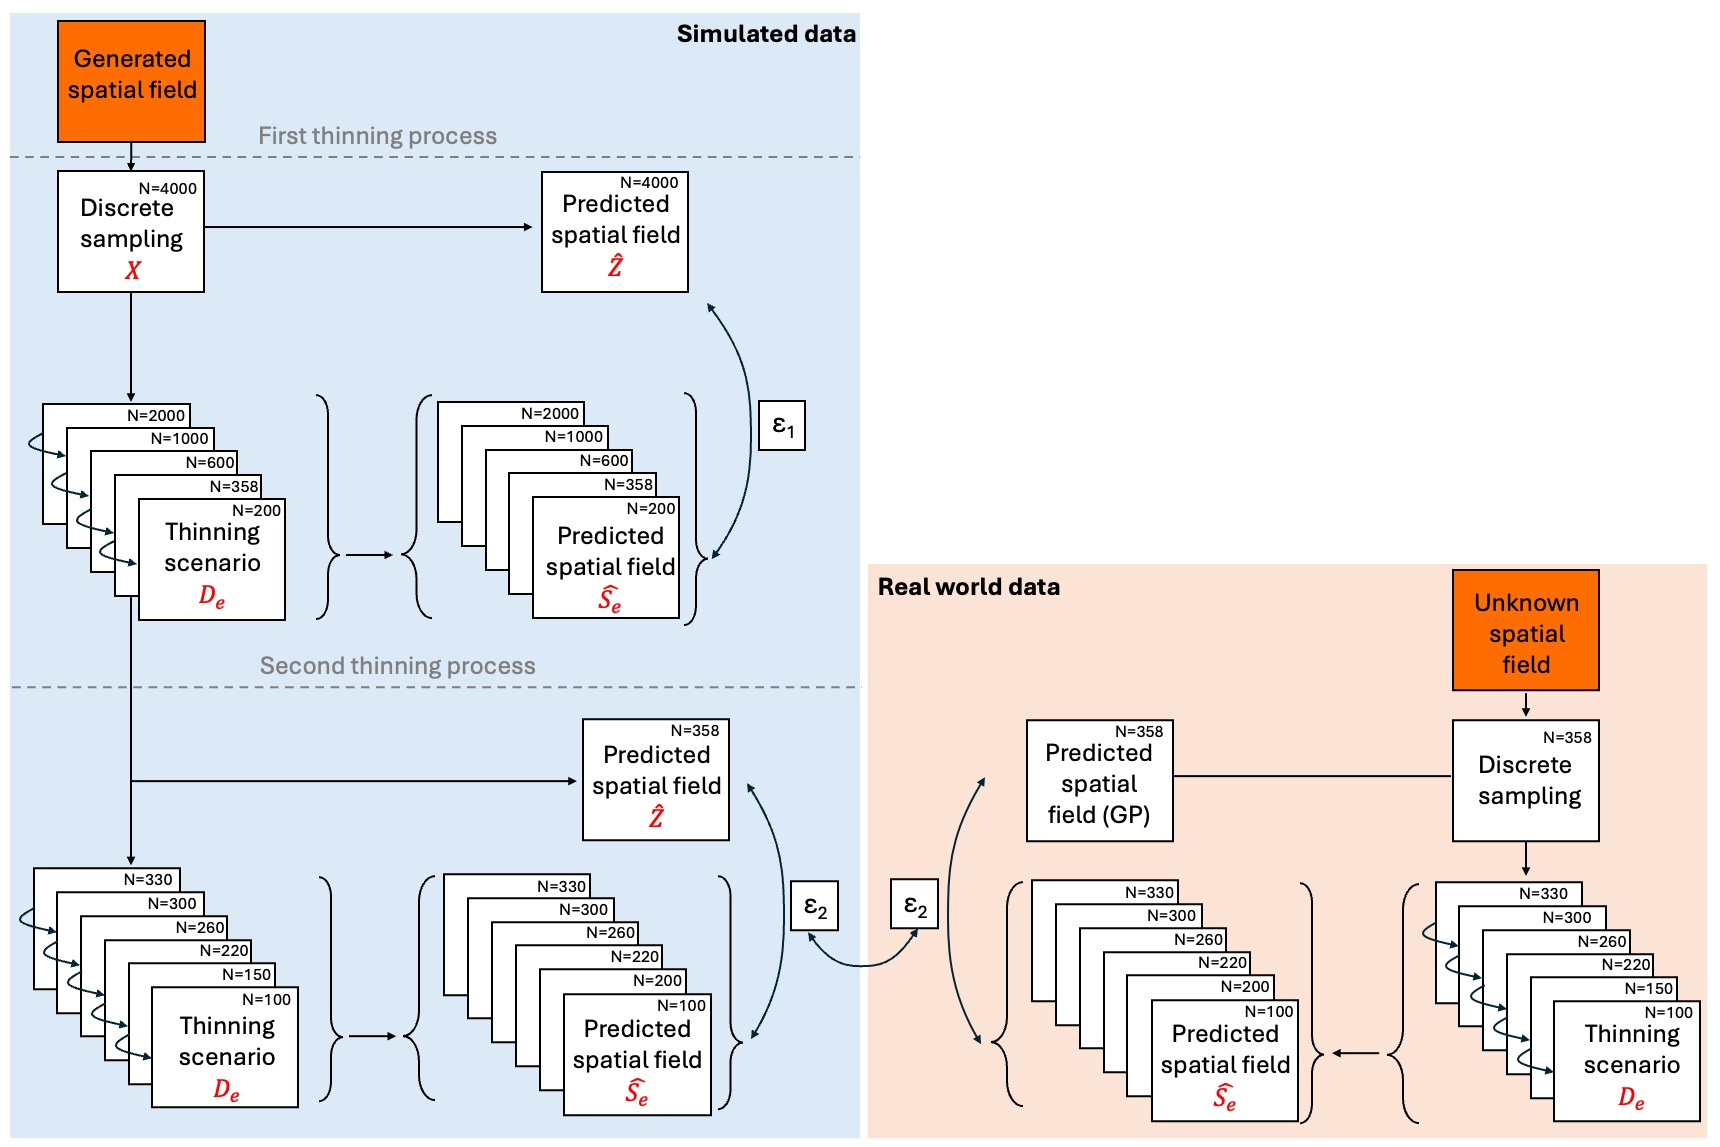
\includegraphics[width=15.5cm]{../../Plots/DAG.jpg}  
\caption{Just figure 1 for now.}
\label{fig:dag}
\end{figure}
\clearpage




















\section{Results}
% Estimation of rho
The estimation of GP parameters ($\rho$ and $\mu$) showed different behaviours with decreasing sampling effort across all levels of spatial autocorrelation (Figures \ref{fig:rho} and \ref{fig:mu}). Regarding the estimation of $\rho$ (Figure \ref{fig:rho}), we observed that as sampling effort decreased, the accuracy of length-scale estimates declined across all simulated $\rho$ values, particularly for simulations with high spatial autocorrelation ($\rho > 500$ km). This trend became more pronounced at lower sampling efforts (e.g., 200 and 358 sampling points), where length-scale estimates exhibited increased variance around the 1:1 line and a general underestimation for simulations with $\rho > 500$ km. Conversely, at higher sampling efforts (e.g., 1000 and 2000 points), length-scale estimates closely approximated the true values with reduced uncertainty. However, a few sporadic overestimations were observed at small $\rho$ values (below 25 km) even at higher sampling efforts, likely due to the limited spatial resolution of the sampling design relative to the rapid spatial variation in these scenarios. 
\textcolor{red}{TODO: maybe I should add some values here to quantify the variance?}

\begin{figure}[tbhp] 
\centering
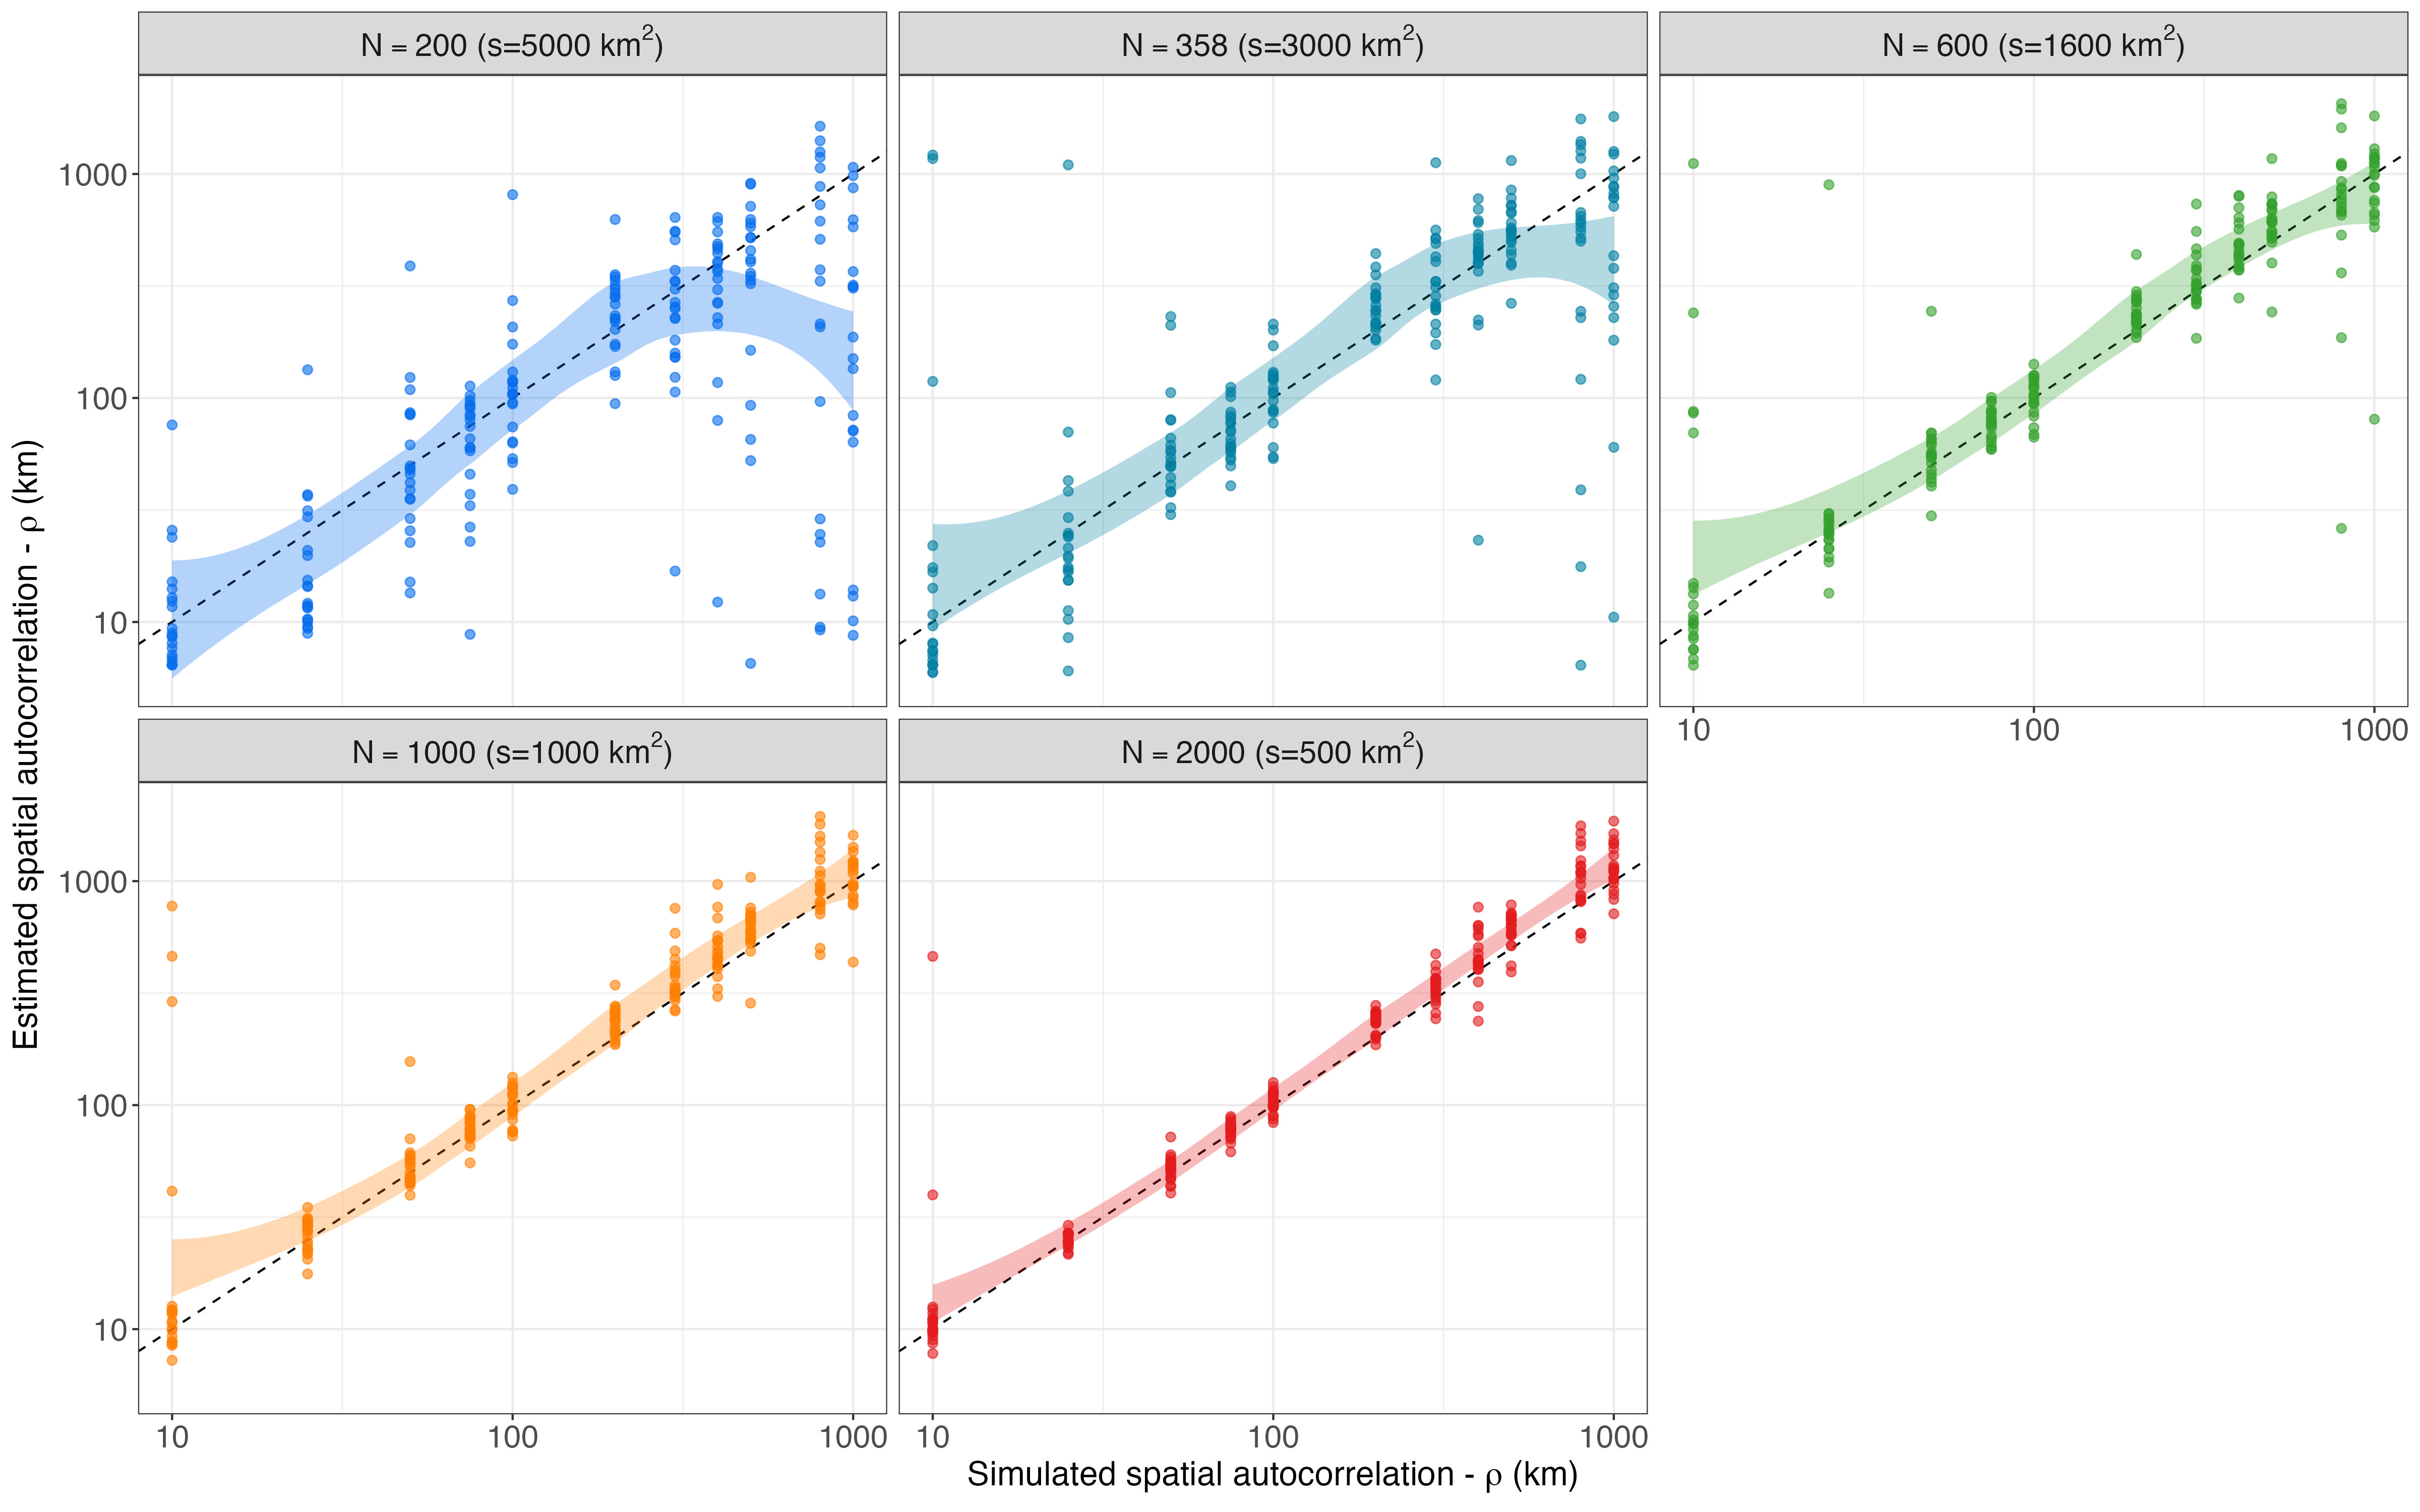
\includegraphics[width=15.5cm]{../../Plots/Figure_1.jpg}  
\caption{Estimated vs simulated spatial autocorrelation parameter ($\rho$) across five sampling-effort scenarios. Each panel and color represents a different sampling effort (number of samples) campaign. The dashed line indicates the 1:1 relationship where estimated values equal simulated values and the grey ribbon represents the 95\% credible interval around the estimates. The accuracy of spatial autocorrelation estimation decreases with the decreasing sampling effort.}
\label{fig:rho}
\end{figure}

% Estimation of mu
Estimates of the global mean ($\mu$; Figure~\ref{fig:mu}) were generally more robust to reductions in sampling effort than the length-scale parameter. Across all sampling effort, estimates of $\mu$ remained relatively accurate, with a small increase in variance at lower sampling efforts (200 and 358 smaples). However, under high spatial autocorrelation -- particularly with $\rho$ above 200 km -- the model showed a systematic pattern of over- and underestimating low and high $\mu$ respectively. This bias produced a characteristic deviation from the expected 1:1 relationship, yielding a slightly tilted relationship trend that reflects the spatial autocorrelation influence across the full range of simulated means. Despite the constrain in our constructed GP model ($\mu >$-5) this pattern was most pronounced for values of $\mu$ below -2 and above 3, suggesting that in high spatially autocorrelated scenarios the model relied more heavily on the prior than on the data when estimating the global mean.

% \clearpage
\begin{figure}[tbhp] 
\centering
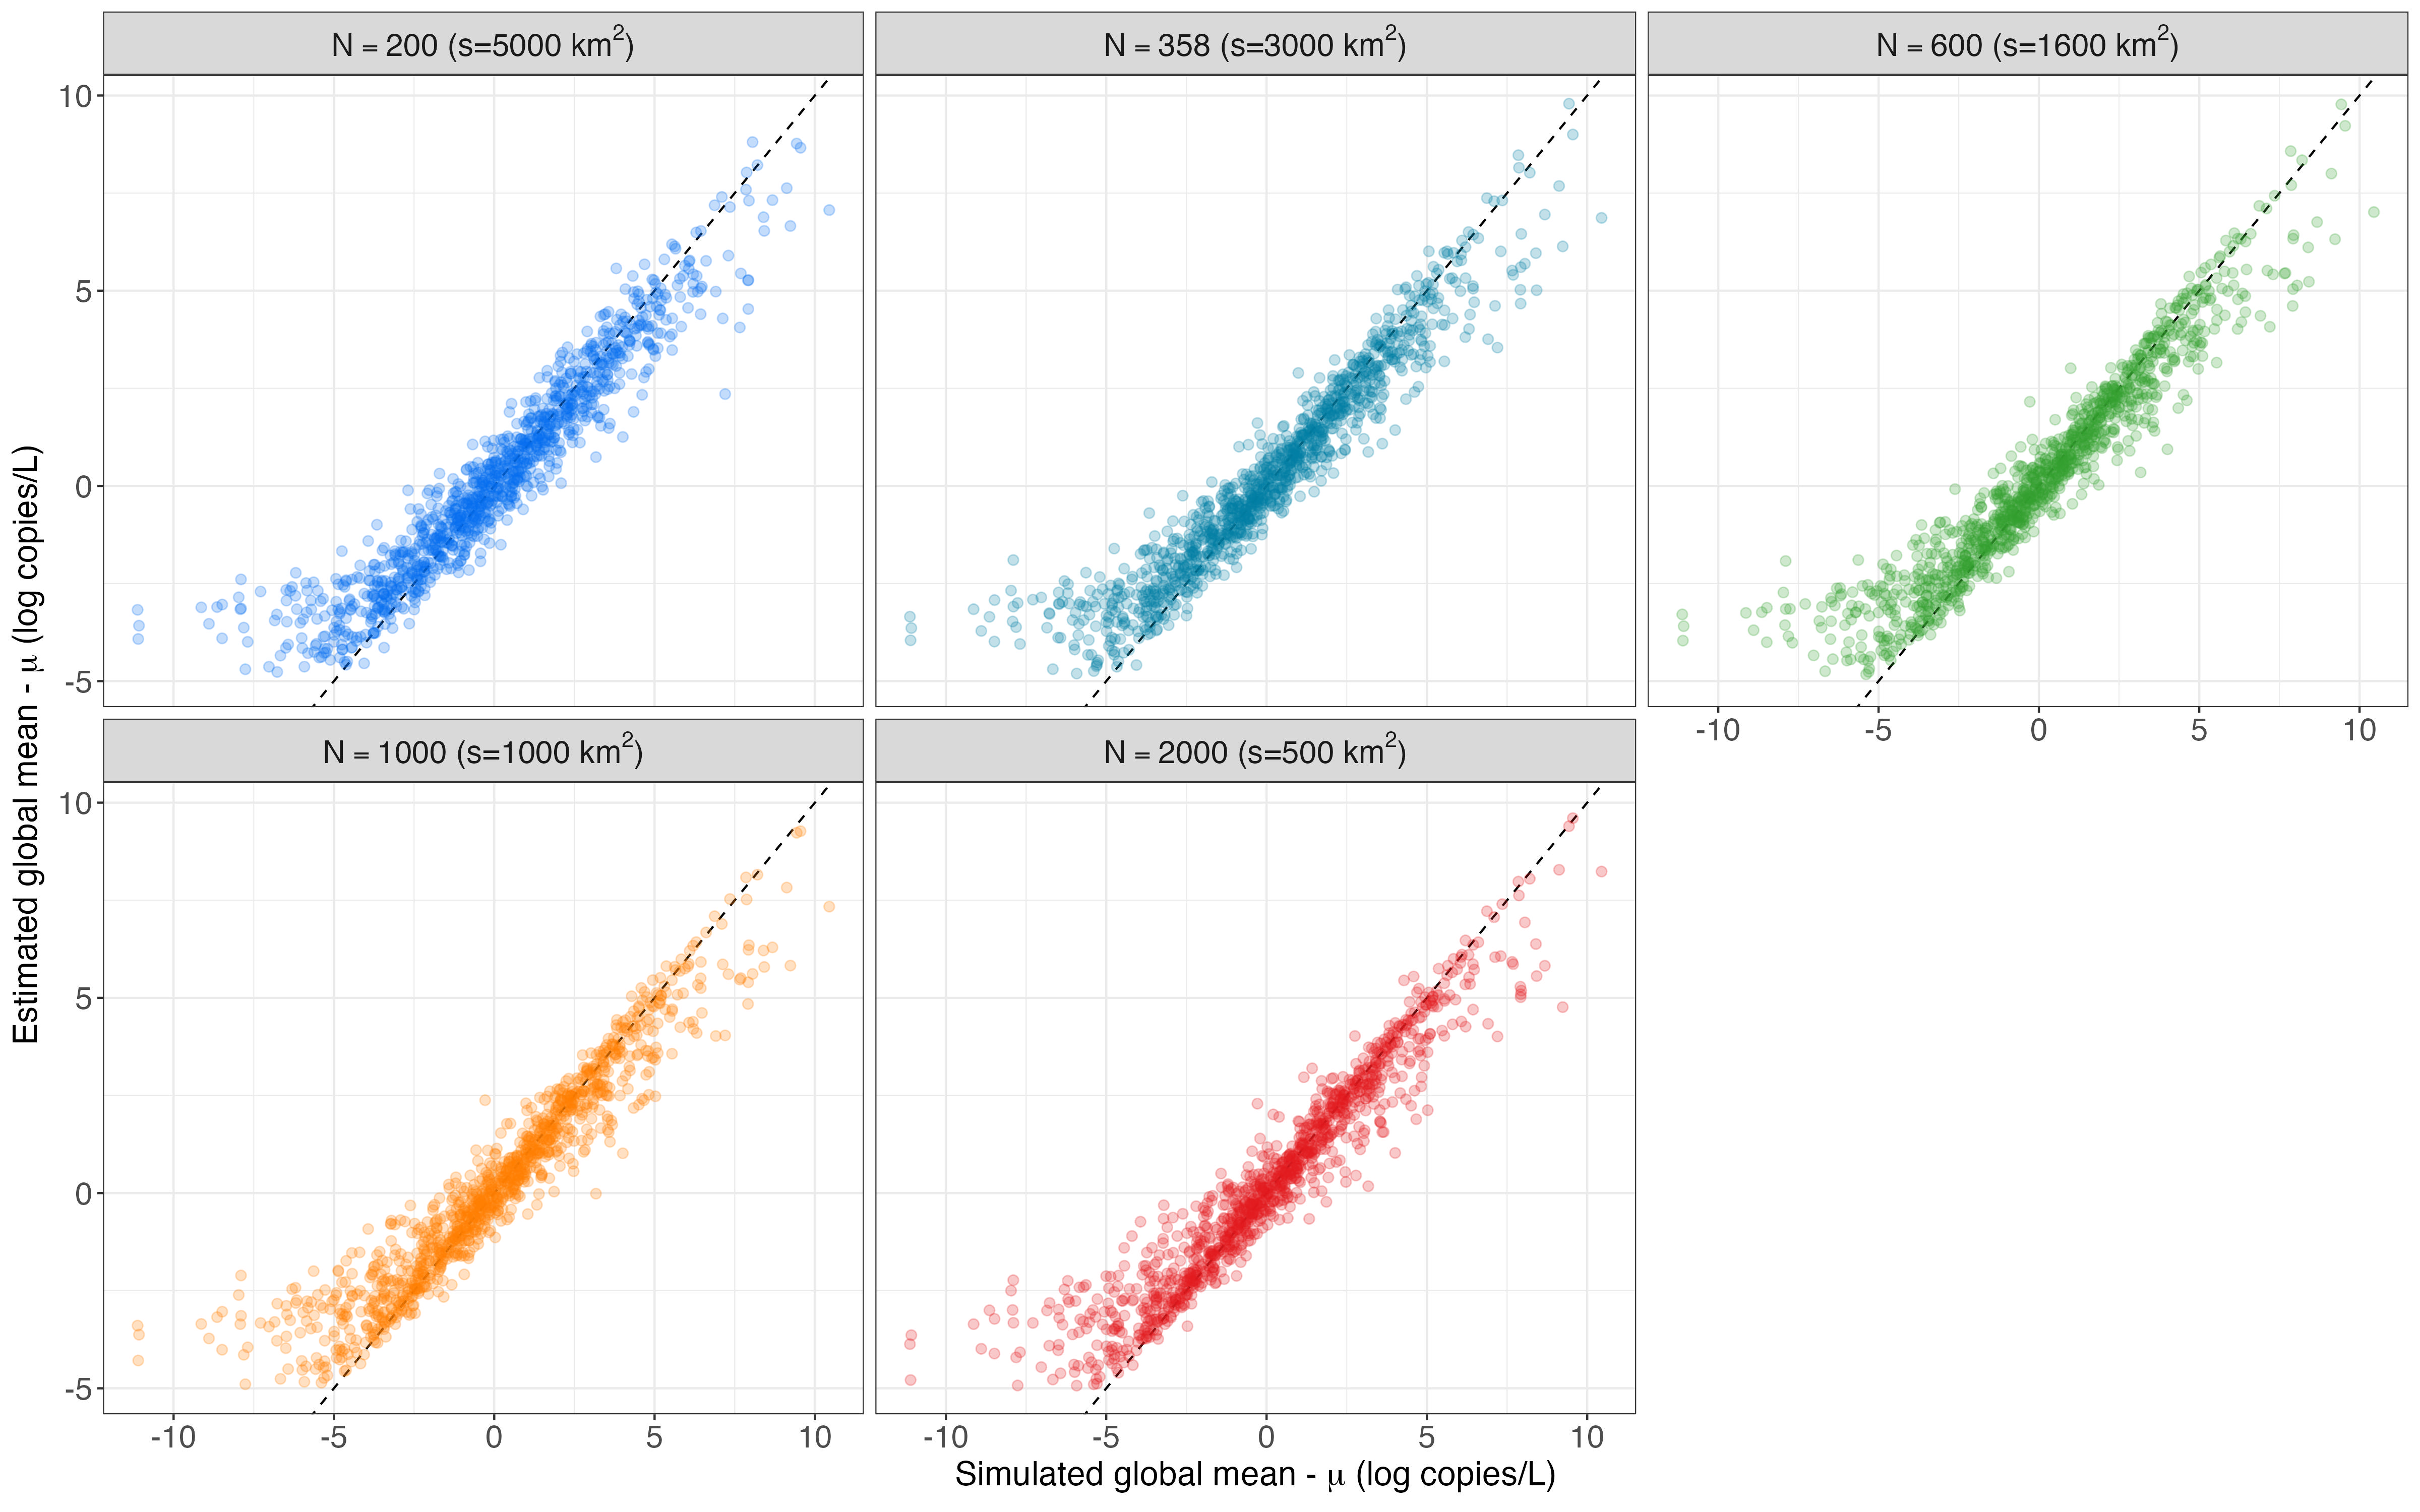
\includegraphics[width=15.5cm]{../../Plots/Figure_2.jpg}  
\caption{Estimates of global mean parameter ($\mu$) across five sampling-effort scenarios. Each panel and color represents a different sampling effort (number of samples) campaign. The dashed line indicates the 1:1 relationship where estimated values equal simulated values and the grey ribbon represents the 95\% credible interval around the estimates. The accuracy of global mean estimation decreases slightly with the decreasing sampling effort.}
\label{fig:mu}
\end{figure}
% \clearpage
% \textcolor{red}{TODO: Add to supplementary the variance of estimating mu across N and also the slope of mu\_est v mu\_sim along the rho values} 


Prediction accuracy, as measured by the mean prediction error ($\epsilon$), improved with greater sampling effort (Figure \ref{fig:epsilon}) and with higher spatial autocorrelation. Mean prediction error ($\epsilon$) increased exponentially as spatial autocorrelation decreased from ca 200 km -- species with lower $\rho$ values exhibited higher prediction errors across all sampling efforts. For instance, at a sampling effort of 600 points, species with spatial autocorrelation values of 25 km had mean prediction errors of 1 indicating that on average every point predicted the eDNA concentration will be off by a factor of 2.72 (for perspective a concentration of 100 copies/L will be predicted between 37-270 copies/L). In contrast, for the same sampling effort (i.e., 600 points) but species with spatial autocorrelation above 500 km had errors below 0.3 indicating an average of over- and underestimation by a factor of 1.35 (for perspective a concentration of 100 copies/L will be predicted between 74-135 copies/L). Additionally, for any given spatial autocorrelation the mean prediction error ($\epsilon$) increased exponentially with decreasing sampling effort.

% \clearpage
\begin{figure}[tbhp] 
\centering
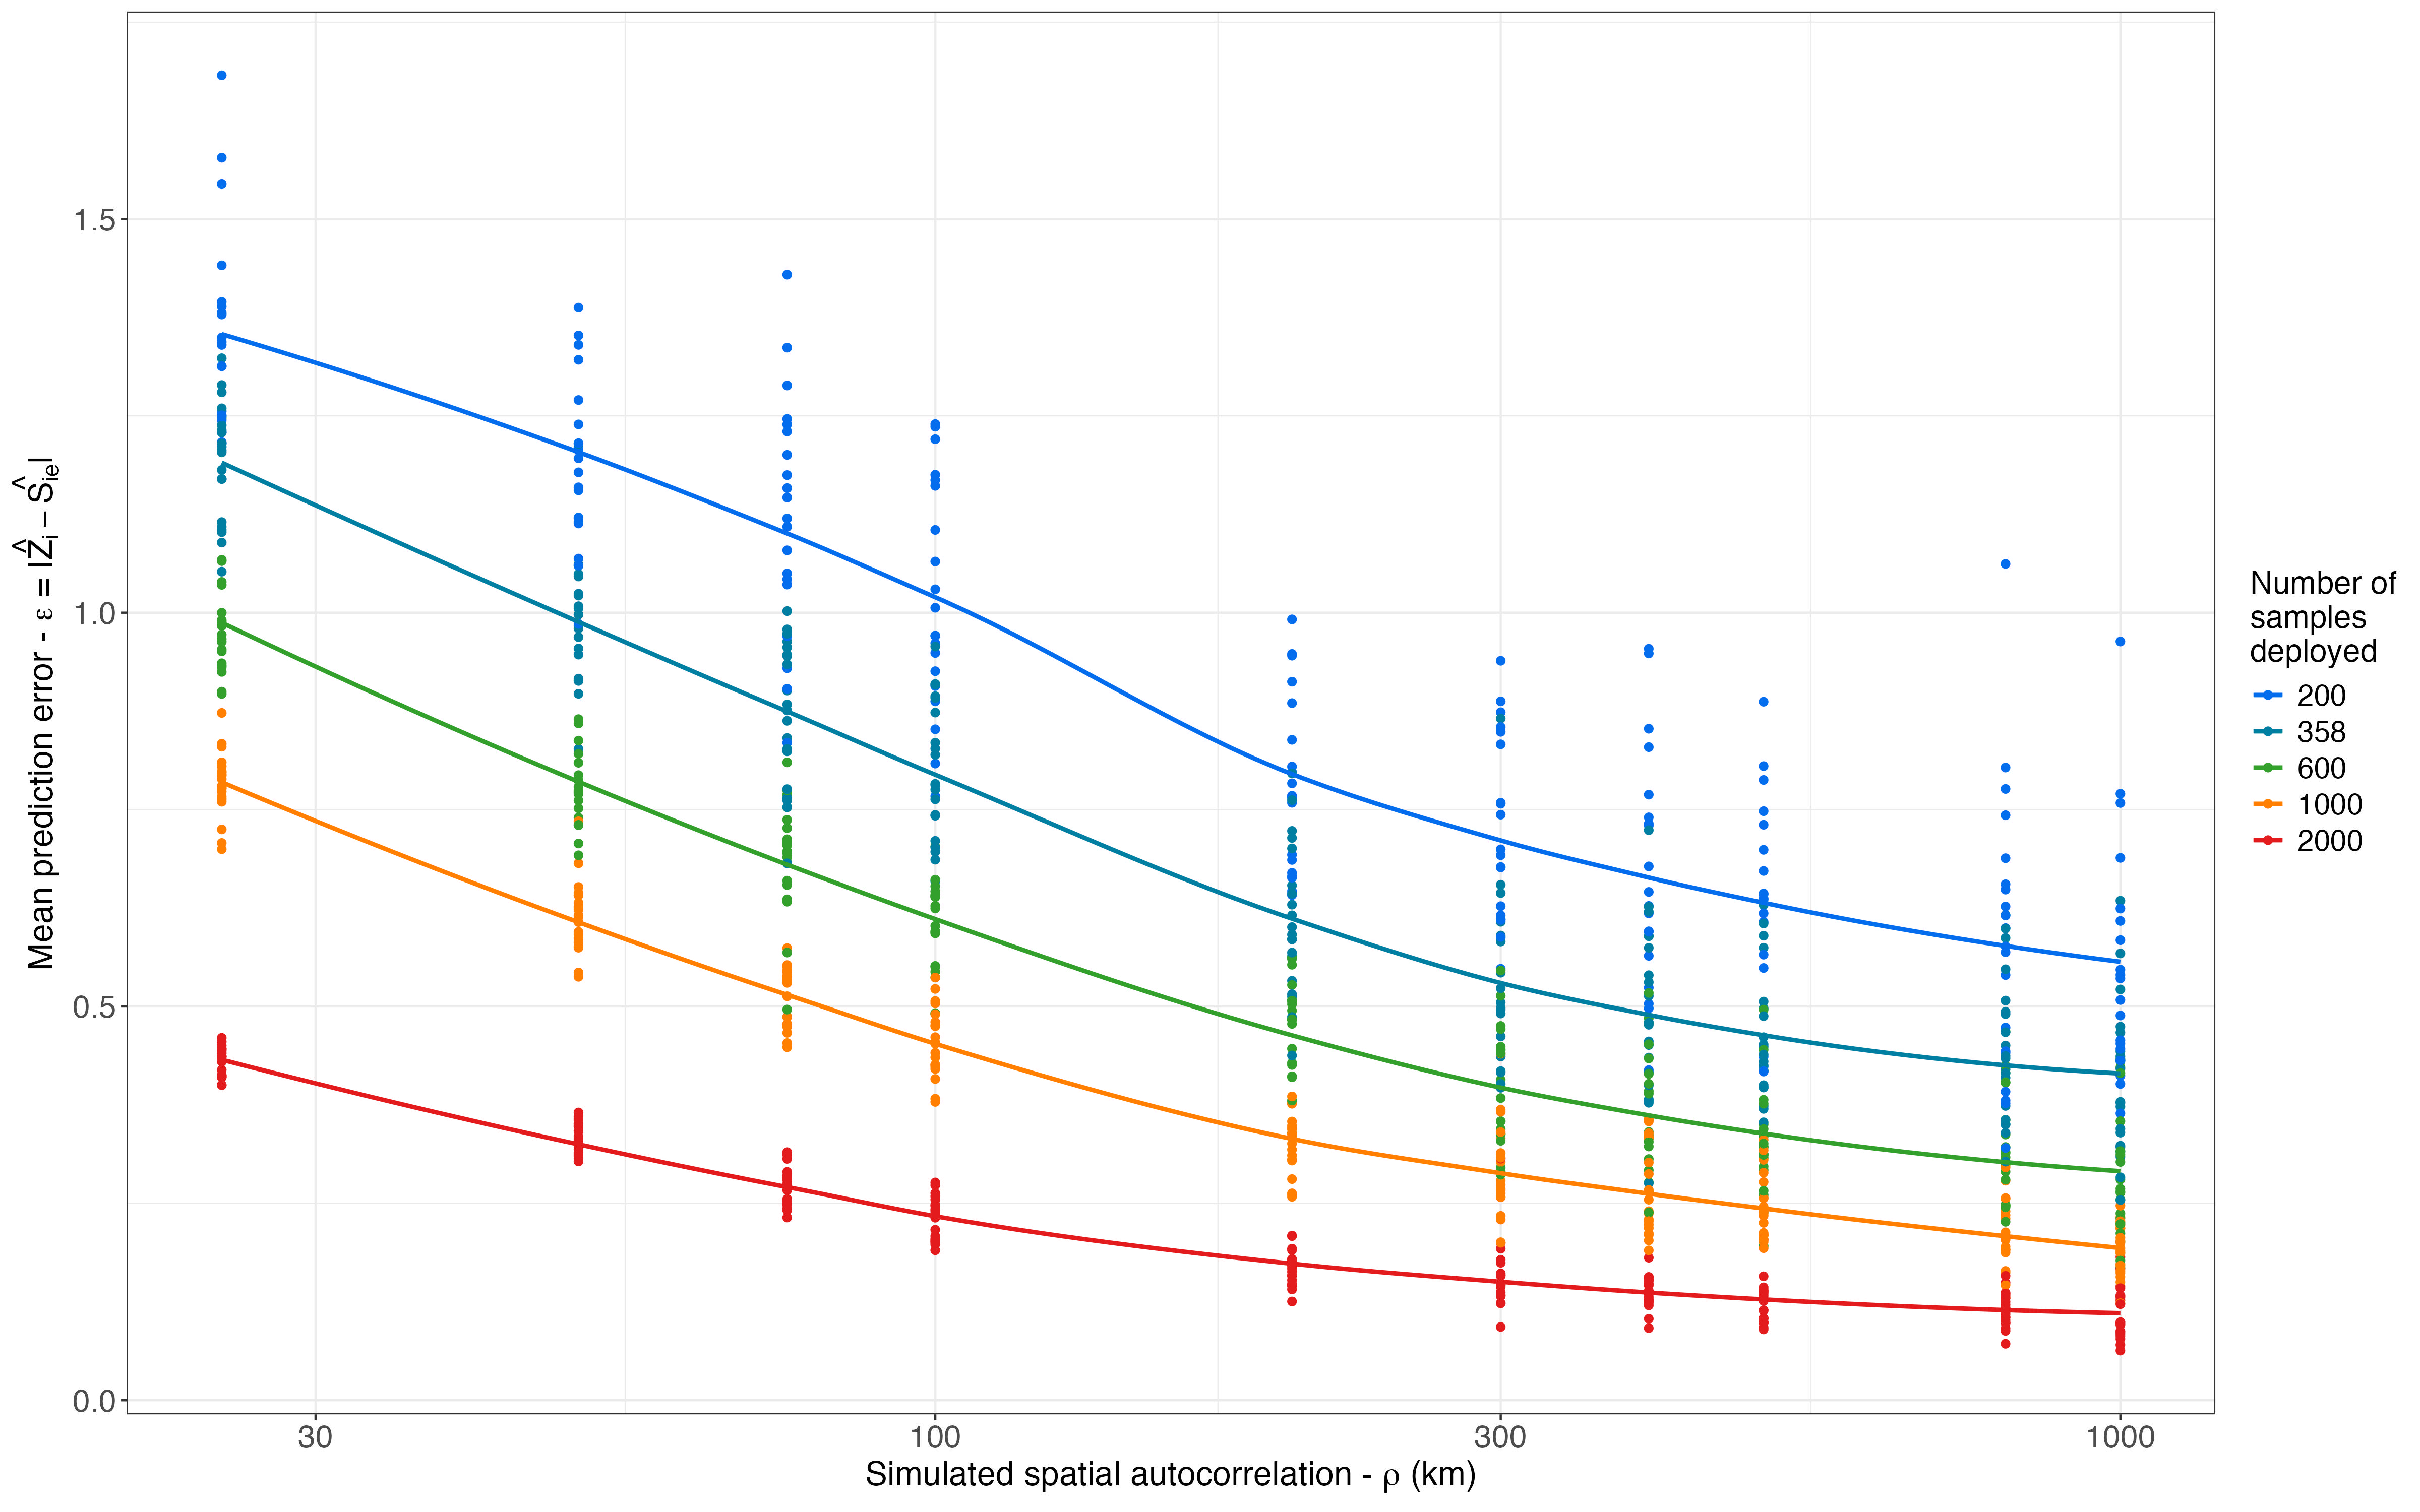
\includegraphics[width=15.5cm]{../../Plots/Figure_3.jpg}  
\caption{Mean prediction error ($\epsilon = \lvert \hat{Z} - \hat{S}_e \rvert$) across five sampling-effort scenarios (indicated by color) for simulated datasets. Prediction error increased with decreasing sampling effort and decreasing as spatial autocorrelation ($\rho$).}
\label{fig:epsilon}
\end{figure}
% \clearpage

The relationship between sampling effort, spatial autocorrelation, and prediction accuracy was further elucidated through the secondary thinning analysis (Figure \ref{fig:epsilon_sp}). Notably, the prediction error patterns observed in the real-world eDNA data were in par with those recovered from the simulated datasets. In both cases, mean prediction error ($\epsilon$) increased as sampling effort decreased and also increased as spatial autocorrelation decreased, but only up to an autocorrelation length of approximately 100 km. Beyond this spatial autocorrelation threshold -- where spatial structure became weak -- prediction error plateaued and exhibited increasingly stochastic behavior, with limited sensitivity to further changes in spatial autocorrelation, indicating that the predicted field $\hat{Z}$ (against which all reduced-effort predicted fields $\hat{S}_e$ are evaluated) was already producing high levels of error (Figure \ref{fig:epsilon}), such that remaining variation in $\epsilon$ appeared purely stochastic. Despite the close correspondence between simulated and empirical patterns, real-world data did exhibit elevated prediction error at intermediate spatial autocorrelation levels (approximately 200 km), suggesting that additional ecological or observational processes may contribute to error in natural systems.


\clearpage
\begin{figure}[tbhp]
\centering
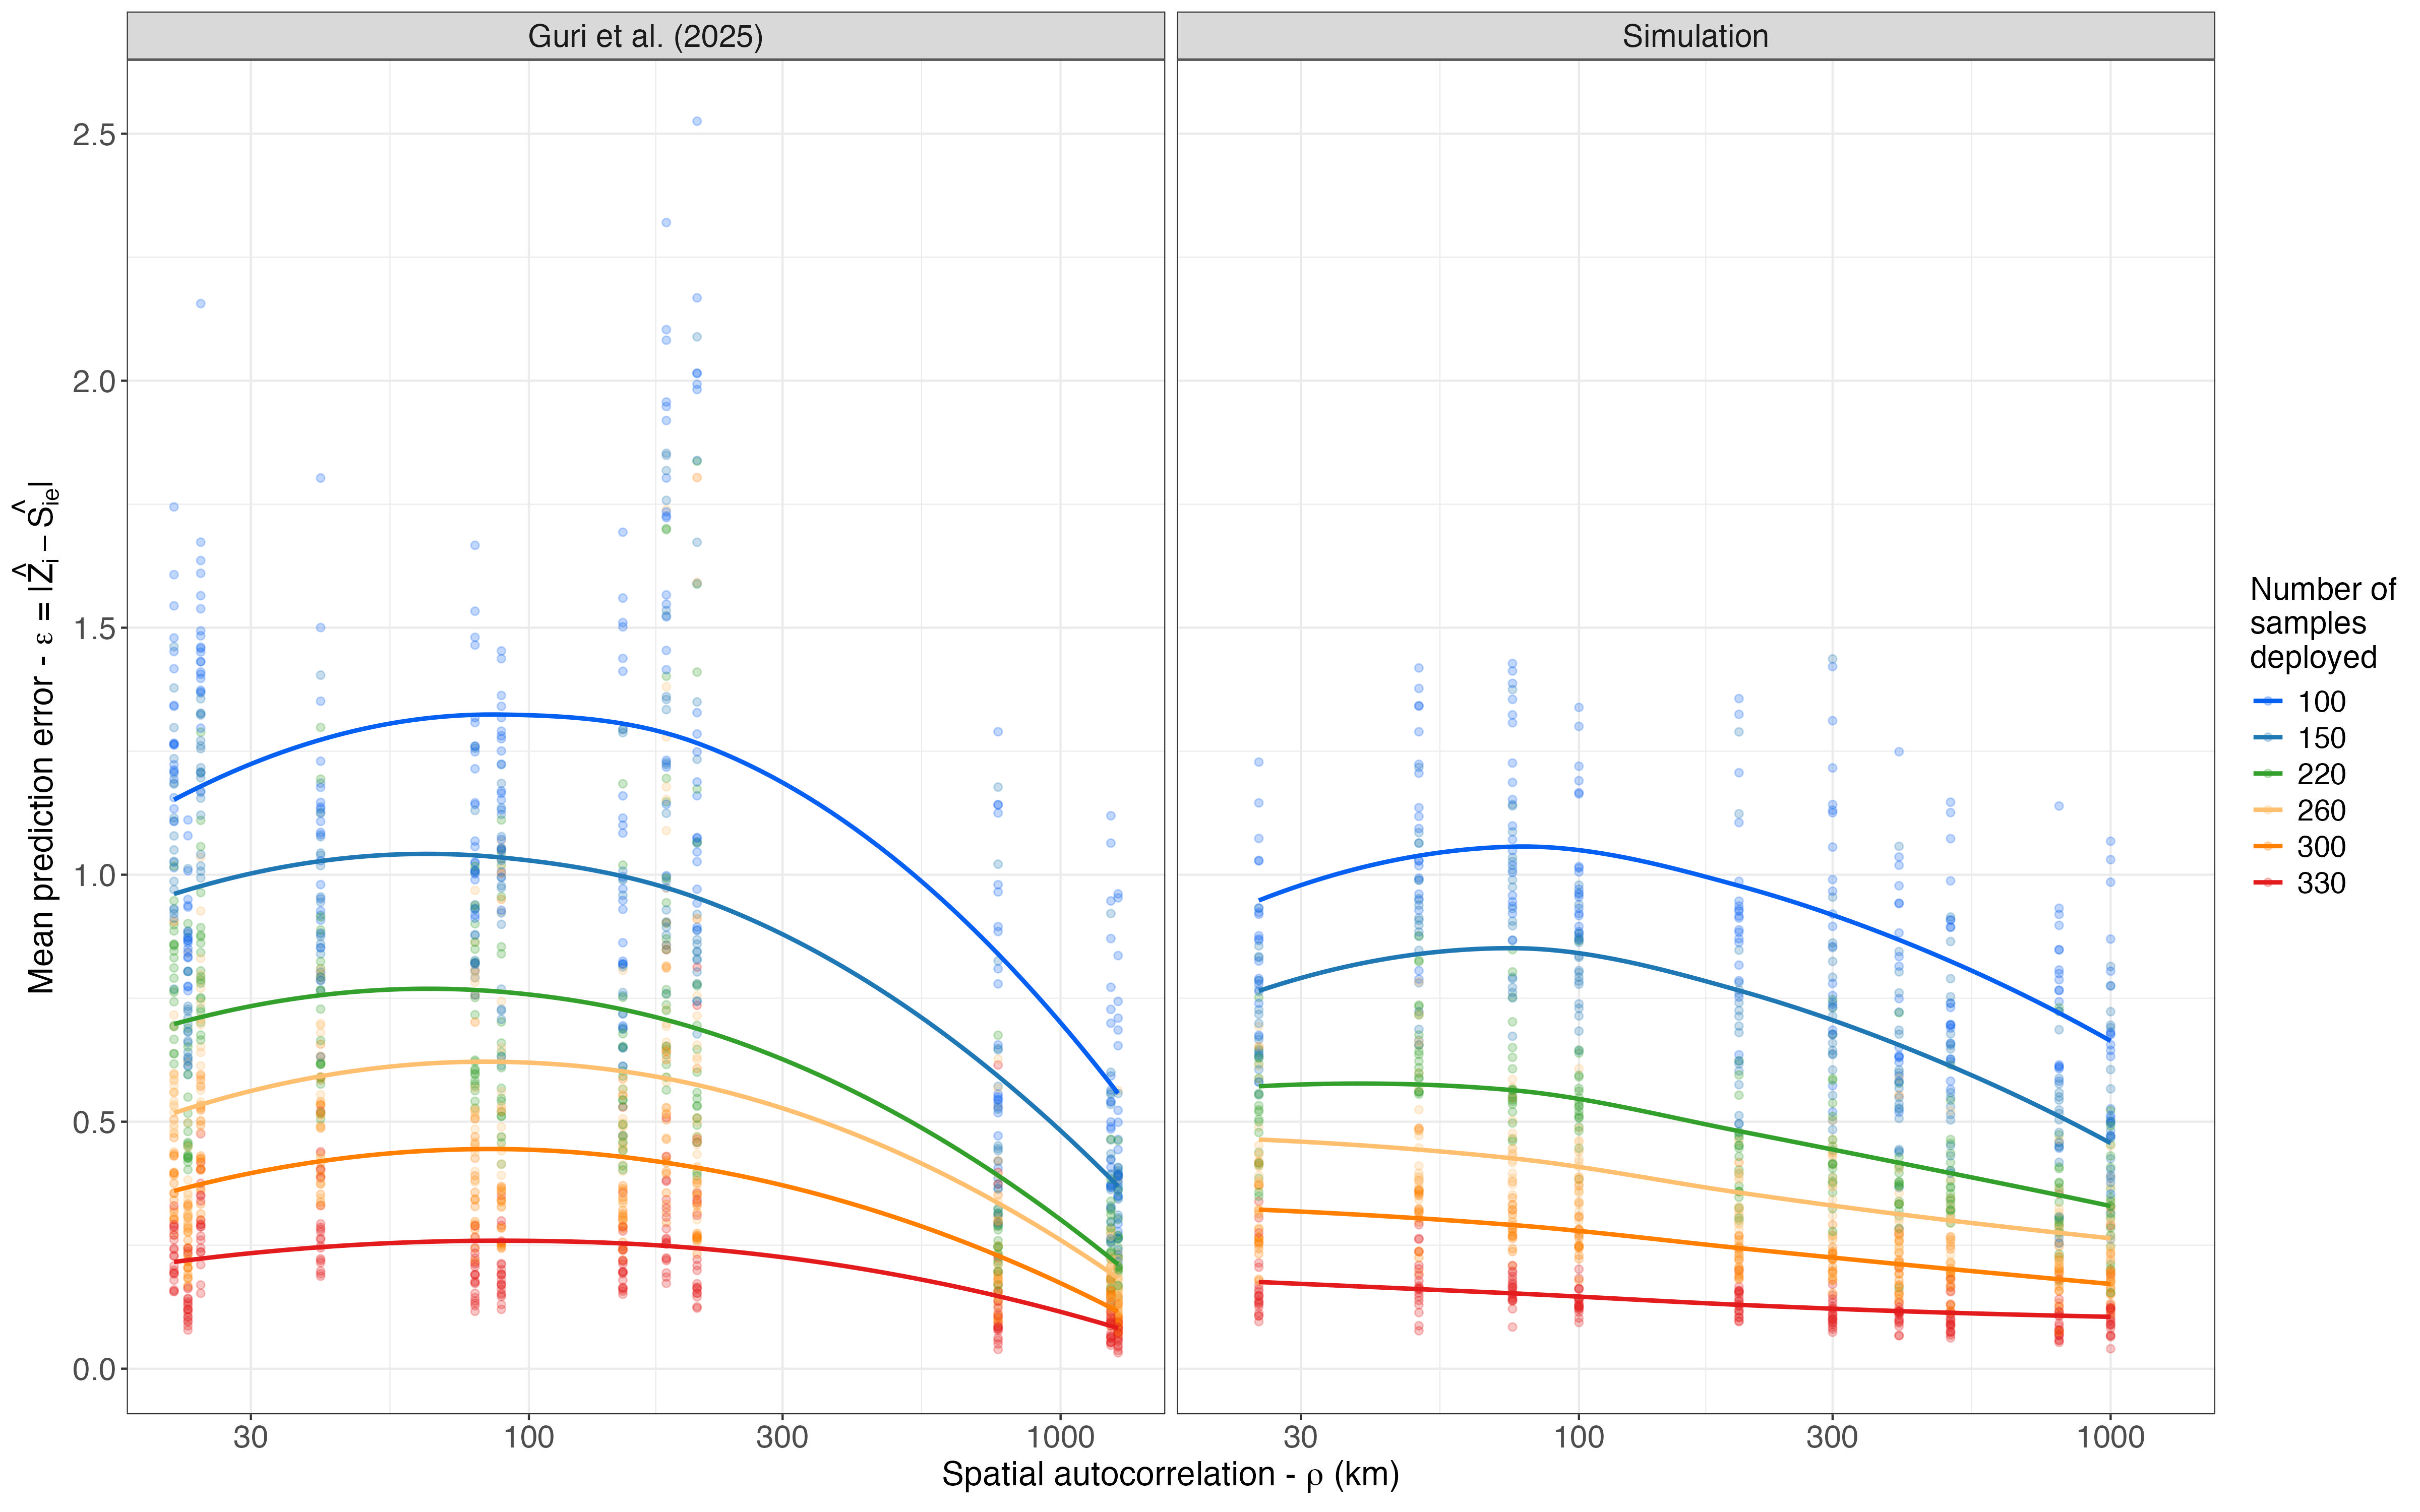
\includegraphics[width=15.5cm]{../../Plots/Figure_4.jpg}
\caption{Mean prediction error ($\epsilon = \lvert \hat{Z} - \hat{S}_e \rvert$) across six sampling-effort scenarios (indicated by color) for real-world eDNA data (left panel) and simulated datasets (right panel). In both cases, prediction error increased with decreasing sampling effort and decreasing spatial autocorrelation ($\rho$) up to approximately 100 km. Beyond this threshold—where spatial structure became weak—prediction error plateaued and exhibited increasingly stochastic variation, with minimal sensitivity to further reductions in $\rho$.}
\label{fig:epsilon_sp}
\end{figure}
\clearpage



















\section{Discussion}


\subsection{Sampling optimisaion}
My raw thoughts:
Other studies do jacknife and rarefaction analysis to check sampling optimisation but they do not have the ground truth to compare against. However doing jacknife or rarefaction would only give you informaiton based on the original sampling design which may be insufficient to recover the spatial structure in the first place as shown in the simulation results. Therefore such approaches cannot reveal information that was never captured. 

Our simulation approach overcomes this limitation by having known parameters and spatial fields to compare against. This allows us to directly quantify how sampling effort influences the recovery of spatial structure and prediction accuracy.

My idea for the discussion structure is to tie each of the three main results to their implications for different ecological and fisheries applications. For people who care about estimating spatial autocorrelation (ecological niche modeling), estimating global mean (stock assessment), and predicting accuracy (species distribution modeling).

\subsection{Ecological niche modeling implications}
\subsection{Stock assessment implications}
\subsection{Species distribution modeling implications}



%use some of these words and language and maybe cite it too
Determining which sampling method is optimal for a given application will depend not only on the monitoring objective, but also on the sensitivity, ease and cost-efficiency of each approach. . achieve a low detection probability, the totality of costs associated with a . The approach presented here allows researchers and managers to assess such trade-offs between sampling methods by quantifying how different parameter values and assumptions affect the cost-efficiency of each sampling technique. Importantly, this approach can be applied to any sampling method or study system where information on detection rates and survey costs is available. This information could come from pilot studies, prior research or could be simulated using sensitivity analyses (where plausible bounds on parameters can be obtained). Our modelling approach could usefully be extended to other emerging technologies such as unmanned aerial vehicles, camera traps and automated recording devices. Such applications will enable researchers and managers to determine the circumstances in which it is worthwhile to adopt novel, but uncertain techniques in lieu of more established sampling methods.
\cite{smart2016}

%maybe use this for stating that the entire budget goes mostly to filed work and very little to dry lab work
Comparing the costs and detection probabilities of optimal trapping and eDNA sampling regimes enabled us to directly compare the cost-efficiency of the two sampling methods across a range of fixed budgets. This analysis revealed that the most cost-efficient sampling method was sensitive to the survey budget, the costs of eDNA primer/probe development and sample processing and the number of positive qPCRs used to designate a water sample as positive for L. v. vulgaris DNA. Environmental DNA sampling was more cost-efficient than bottle-trapping across a range of small to intermediate budgets when primer/probe development and sample processing costs were low (i.e. low-cost scenario) and when 1/4 or 2/4 positive qPCRs were used to designate a water sample as positive for L. v. vulgaris DNA (Fig. 2). This disparity in cost-efficiency was greater when the detection rate differed more markedly between the two sampling methods (Fig. 3).
\cite{smart2016}




\clearpage
\bibliography{Bib.bib}
\clearpage











\section{Appendix}

\begin{figure}[tbhp] 
\centering
\includegraphics[width=15.5cm]{../../Plots/Figure_2_extended.jpg}  
\caption{Just figure 2 for now.}
\label{fig:mu_rho_N}
\end{figure}
\clearpage


\end{document}

